\subsection{Corticospinal Segmentation}
\label{subsec:experiments_segmentation}
After creating the tractography and vidation, the correct tractography is ready for segmentation. In this project, we focus on the ALS disease. Due to the fact that the ALS disease is involved to the CST (Corticospinal Tracts), the segmentation task is only interested in the CST segmentation. 

Actually, segmentation CTS requires a lot of experiments and high preciseness of the anatomic brain. For that reason, this step is going on with the help from doctor Nivedia by using our Sphagetti software. The segmentation procedure can be described as the following steps:
\begin{itemize}
	\item Choose some bundles representing for the main direction of the CST
	\item Expand to more detail bundles (by changing the value of distance)
	\item Remove bundles not in the region of interest or not following the direction of CST
	\item Looping until all the chosen tracks are visualized (the distance is 01)
\end{itemize}

\begin{figure}
  \centering
  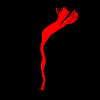
\includegraphics[bb=0 0 140 150]{201CTS1Mleft_1.png}
  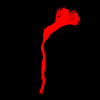
\includegraphics[bb=0 0 140 150]{201CTS3Mleft_1.png}%[bb=0 0 200 300]
  \caption{The left CTS segmentation of control 201 in the dataset ALS\underline{ }Nivedita. The left image is the segmentation from the 1M tractography and has $154$ tracts. While the right is one from 3M tractography and the number of tracts is $487$.}
  \label{fig:CTS_201_left}
\end{figure}

The result of CTS segmentation contains the index of the tracts, and is saved in subfolder Segmentation. For each tractography of every subject/control, the CTS segmentation includes two files correspondingly to the left and the right of the brain. Because we have three tractography for each subject/control ($10K, 1M and 3M$), in total there are six CTS segmentation files for each subject/control. An example of the result is showed in the figure \ref{fig:CTS_201_left}.


